\prob
{
    Let $G$ be the directed graph shown in the next figure 
		    \begin{center}
                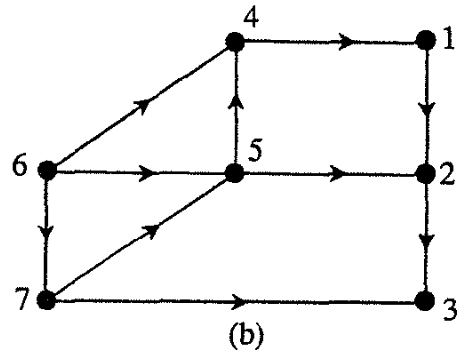
\includegraphics[width=5cm]{Test2/Problem13/Figure2_17.png}
            \end{center}\pn
		and let $M = L(G, B_0)$ where $B_0 = \{1,2,3\}$. 
    \begin{enumerate}[label=(\roman*)]
        \item   Find geometric representations for $M$ and $M^*$.
        \item   Give a presentation for the transversal matroid $M^*$.
        \item   Reverse the directions on the arcs $(5,4)$ and $(7,5)$ of $G$
                and repeat $(i)$ and $(ii)$.
    \end{enumerate}
}
\begin{proof}
    \begin{enumerate}[label=(\roman*)]
        \item $\,$\pn
                 \begin{figure}[H]
                    \begin{center}
                        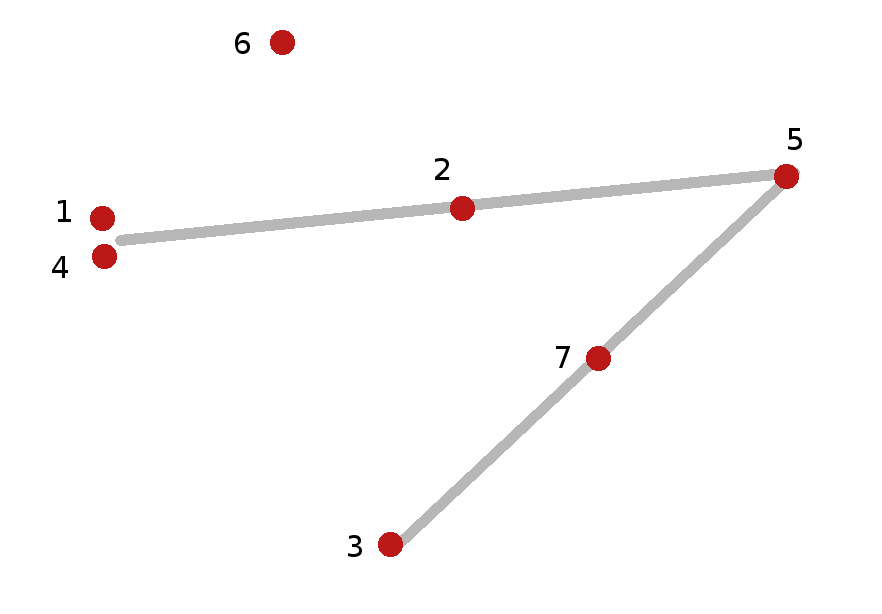
\includegraphics[width=8cm]{Test2/Problem13/GraphicRepresentationM.png}
                    \end{center}                            
                    \caption{Geometric representation for $M$}
                    \label{t2:p13_GraphicRepresentationM.png}                        
                \end{figure}\pn    
                
        \item  Following the method exposed in the book, the family $\mathcal{A} = \{\{1, 4\}, \{2, 4, 5\}, \{4, 5, 6, 7\}, \{3, 5, 7\}\}$
                is a presentation for $M^*$.
                
        \item As the directions inside $B_0$ doesn't affect the gamoid, to invert $(5,4)$ and $(7,5)$
                produces exactly the same matroid but exchanging the labels of $4$ and $7$.\pn
    \end{enumerate}
\end{proof}